\section{A two dimensional example}
\label{sect:two_dimensional_example}
\par
In this example we aim to create a mesh in a rectangle, as shown in figure
\ref{fig:shot16}.
%\begin{figure}[htbp]
%\centering
%\includegraphics[width=1.0\textwidth]{../figures/2d-example-mesh.png}
%\caption{Mesh on the rectangle}
%\label{fig:2d-example-mesh}
%\end{figure}
The following steps will be taken:
\begin{enumerate}
  \item Set up the geometry. The graphical user interface of Gmsh is used to carry out the following
           steps:
  \begin{enumerate}
    \item Create the two points on the left-hand side of the rectangle.
    \item Connect the two points with a line
    \item Extrude the line to form the rectangle.
  \end{enumerate}
  \item Define physical groups. Defining physical groups results into numerical ID's being assigned to
           each group. Fluidity uses these ID's to apply boundary conditions.
  \item Customise the geometry. A subset of the Gmsh scripting language is introduced and modifications
           will be made to the geometry script.
  \item Produce a mesh.
\end{enumerate}
The following sections go through the above steps, in great detail.

\subsection{Setting up the geometry}
\label{ssect:setting_up_geometry}
\par
\par
Run gmsh on the command line, storing the geometry in \lstinline{channel.geo}:
\begin{lstlisting}
gmsh channel.geo
\end{lstlisting}
\par
Create the points at the left-hand-side of the rectangle:
\begin{enumerate}
  \item Go to the top-most level of the Geometry module in the menu window.
  \item On the menu window click on \lstinline{Elementary entities > Add > New > Point} , see
        figure \ref{fig:basic_interaction}. The ``Contextual Geometry Definitions'' window will
        appear at the point tab, as shown in figure \ref{fig:creating_a_point}.
        Note that  moving the cursor over the graphic window will cause the coordinates shown in
        the Contextual Geometry Definitions window to change. While the user is allowed to specify
        points using this interactive \& graphical interface, we will directly enter the point
        coordinates on the Contextual Geometry Definitions window. Doing so allows for more accurate
        control of the point coordinates.
  \item Add a point at $(x,y,z)=(0,-1,0)$, with a characteristic mesh element size of $1.9$: Modify the
        parameters in the Contextual Geometry Definitions window, to match those shown in
        figure \ref{fig:creating_a_point} and click on ``Apply'' (on the same window). Be careful not
        to move the cursor over the graphic window, as it will change your coordinates.
  \item Add another point at $(0,1,0)$
  \item Close the Contextual Geometry Definitions window.
\end{enumerate}
\par
Create a line representing the left-hand edge of the rectangle:
\begin{enumerate}
  \item Click on \lstinline{Geometry (G) > Elementary entities > Add > New > Straight line}
  \item Choose the starting point of the line segment on the graphic window. Note that the
        starting point should now be coloured red. If not, try selecting it again.
  \item Choose the ending point of the line segment. If the point selection is successful,
        the straight line segment should appear in the graphic window, and you should have
        something similar to the left-most panel in figure \ref{fig:gmsh_extrusion}.
  \item Press ``q'' on your keyboard.
\end{enumerate}
\begin{figure}[htbp]
 \centering
  \includegraphics[width=1.0\textwidth]{../figures/navigating_to_extrusion.png}
  \caption{Directing Gmsh to extrusion.}
  \label{fig:gmsh_extrusion}
\end{figure}
\par
Note that one could simply create all four points at the rectangle vertices and then simply draw the
lines to from the rectangle sides. However, extrusions  are used below as it demonstrates more features
of Gmsh and it facilitates the creation of a structured mesh:
\begin{enumerate}
  \item Go to the top-most level of the Geometry module in the menu window.
  \item Click on \lstinline{Elementary entities > Extrude > Translate > Line},
        as indicated in figure \ref{fig:gmsh_extrusion}. The Contextual Geometry Definitions window will
        appear, set to the Translation tab, as shown in the left panel of figure \ref{fig:extrusion}
  \item Modify the parameters in the Contextual Geometry Definitions window to specify an extrusion
        along the $x$-direction of $10$ length-units, as shown in the left panel of
        figure \ref{fig:extrusion}.
  \item Click on the line we previously drew on the graphical window, it should be highlighted in red,
        as shown in the left panel of figure \ref{fig:extrusion}.
  \item Press the key ``e'' on your keyboard, a rectangle should appear in the graphical window, as shown
        in the right panel of figure \ref{fig:extrusion}.
  \item Close the Contextual Geometry Definitions window.
\end{enumerate}
\begin{figure}[htbp]
 \centering
  \includegraphics[width=1.0\textwidth]{../figures/extrusion.png}
  \caption{Extruding a line to form a rectangle.}
  \label{fig:extrusion}
\end{figure}
\par
%The following was not strictly necessary and was commented out. However it is not deleted, as it may
%be re-instated in a future version.
%The extrusion also defines a surface, the following steps show how to edit some of the gmsh options, so
%as to make Gmsh to highlight plane surfaces:
%\begin{enumerate}
%  \item On the menu bar of menu window of Gmsh click on ``Tools'' and select ``Options'', as highlighted
%        in the right panel of figure \ref{fig:gmsh_basic_options}. The ``Options'' window will appear.
%  \item In the Options window, select  the ``Visibility'' tab. On the side list select ``Geometry'' and
%        if not already activated, activate ``Surfaces'' (see left panel of figure
%        \ref{fig:gmsh_basic_options}).
%\end{enumerate}
%The interior of the square should now be marked with a gray, chain line as shown in
%figure \ref{fig:gmsh_basic_options}
%\begin{figure}[htbp]
% \centering
%  \includegraphics[width=1.0\textwidth]{../figures/gmsh_basic_options.png}
%  \caption{Changing the Gmsh options to highlight defined surfaces on the graphic window.}
%  \label{fig:gmsh_basic_options}
%\end{figure}

\subsection{Physical groups: boundaries and regions}
\label{ssect:2d_physical_groups}
\par
In order to apply boundary conditions it is necessary to specify ``Physical groups'' to which the boundaries belong. Since Gmsh will only export to a file those elements which are associated with a physical entity, it is also necessary to identify the interior of the domain with a physical group. Declare a physical surface over the interior of the rectangle as follows:
\begin{enumerate}
  \item Go to the top-most level of the Geometry module in the menu window.
  \item Click on \lstinline{Geometry > Physical group > Add > Surface}.
  \item Gmsh will highlight any surfaces with grey broken lines, see figure \ref{fig:shot15}
        for example.
  \item Select the plain-surface created in section \ref{ssect:setting_up_geometry}, by clicking on the
        broken grey line.
  \item Press ``e'' on your keyboard to end the selection, and then ``q''.
\end{enumerate}
Then declare physical lines from the edges of the rectangle as follows:
\begin{enumerate}
  \item On the menu window of Gmsh click on ``Line'', pick the top side of the rectangle and
        press ``e'' on your keyboard to end the selection.
  \item Pick the top side and the bottom side of the rectangle and press ``e'' on your keyboard to
        end the selection.
  \item On the menu window of Gmsh click on ``Line'', pick the left-hand side of the rectangle and
  \item Repeat the above step, selecting the right-hand-side of the rectangle.
  \item press ``q'' to exit the selection mode.
\end{enumerate}

\subsection{Final customisation of the geometry}
\label{ssect:2d_geo_fine_tuning}
\par
So far, we have been using the graphical user interface to create a simple geometry. we will now
use a less-graphical oriented approach to adjust some important details. At the beginning of the
section Gmsh was invoked using file \lstinline{channel.geo}. The file \lstinline{channel.geo}
 includes a set of declarations that allow Gmsh to reconstruct the geometry, effectively allowing the user
to ``save'' the geometry. Since the \lstinline{channel.geo} file is an ASCII file, any text editor can be
used to edit it, however, we will here use the text editor invoked by Gmsh itself:
\begin{enumerate}
  \item Go to the top-most level of the geometry module in the Gmsh menu window.
  \item Click on \lstinline{Edit}, a text editor instance (usually emacs) will open the file
        \lstinline{channel.geo}, as shown in figure \ref{fig:shot15}.
\end{enumerate}

\begin{figure}[htbp]
 \centering
  \includegraphics[width=1.0\textwidth]{../figures/shot15}
  \caption{The Gmsh windows with the text editor invoked on \lstinline{channel.geo}}
  \label{fig:shot15}
\end{figure}
\par
The file contents should be identical to the left hand-side of the listing below. The numbers present
on the left hand-side of the listings are added here for ease of reference. The \lstinline{.geo} files
are script files containing comments and expressions. Expressions can be further classified into 
string-expressions, floating-point expressions Loops \& Conditionals as well as other categories,
listing the categories is beyond the scope of this tutorial (however, the interested reader can find
the full documentation at \url{http://geuz.org/gmsh/doc/texinfo/gmsh.html#General-tools}). The expressions
of interest to this tutorial are commands that define geometrical objects. So, before the reader proceeds
with editing the file contents, we briefly describe the commands and the syntax of comments.
\begin{itemize}
  \item Lines preceded by \verb$//$ are comment lines and are ignored by Gmsh as it reads the file.
        Also any part of a script file between \verb$/*$ and \verb$*/$ is treated as a comment.
  \item Commands must terminate with \lstinline{;}, otherwise Gmsh assumes that the command is
        continued in the line below (see lines $5$ and $6$).\footnote{Also note that at the end of line
        $7$ a semi-colon should be present. Currently, its absence does not seem to affect Gmsh.}
  \item Commands such as those in line $1$, clearly create a point, and:
  \begin{itemize}
    \item Assign the point-ID in the round brackets on the left-hand-side of the expression to the
          point with coordinates specified by the first three numbers in the braces.
    \item Assign the fourth number in the braces as characteristic mesh size.
  \end{itemize}
  \item Commands such as those in line $3$, clearly create a line segment, and:
  \begin{itemize}
    \item Assign the line-ID in the round brackets on the left-hand-side of the expression to the
          line with endpoint specified by the point-IDs in the braces.
  \end{itemize}
  \item The extrusion command in line $5$ created the three remaining lines of the rectangle, as well
        as the plane surface
\end{itemize}

Edit the file, so as to match the right hand side listing.\\
\begin{minipage}[t]{0.48\textwidth}
\begin{center}
\lstinline+channel.geo+ file as produced by
GUI.
\end{center}
\lstset{numbers=left}
\begin{lstlisting}
Point(1) = {0, -1, 0, 1.9};
Point(2) = {0, 1, 0, 1.9};
Line(1) = {1, 2};

Extrude {10, 0, 0} {
  Line{1};
}
Physical Surface(11) = {5};
Physical Line(16) = {4, 3};
Physical Line(17) = {1};
Physical Line(18) = {2};
\end{lstlisting}
\lstset{numbers=none}
\end{minipage}
\hfill
\begin{minipage}[t]{0.48\textwidth}
\begin{center}
\lstinline+channel.geo+ file after
fine-tuning.
\end{center}
\lstset{numbers=left}
\begin{lstlisting}
Point (1) = {0, -1, 0, 1.9};
Point (2) = {0, 1, 0, 1.9};
Line (1) = {1, 2};

Extrude {10, 0, 0} {
  Line{1};Layers{20};
}

// Volume number for whole domain.
Physical Surface (1) = {5};
// Top and bottom of the box.
Physical Line(333) = {3,4};
// Left wall
Physical Line(666) = {1};
// Right wall
Physical Line(444) = {2};
\end{lstlisting}
\lstset{numbers=none}
\end{minipage}\\
In particular the following changes should be made:
\begin{enumerate}
  \item Append \verb$Layers{20};$ to line $6$. This instructs Gmsh to organise the mesh in $20$
        layers, normal to the extrusion direction.
  \item In line $9$ change \lstinline{Physical Line(16)} to \lstinline{Physical Line(333)}
  \item In line $10$ change \lstinline{Physical Line(17)} to \lstinline{Physical Line(666)}
  \item In line $11$ change \lstinline{Physical Line(18)} to \lstinline{Physical Line(444)}
  \item Insert comment-lines to match the left-hand-side listing above.
\end{enumerate}
Save the file and close the editor window. Click on \lstinline+Reload+ in the Gmsh menu window, Gmsh needs to read the updated file. You are now ready to generate a mesh.

\subsection{Producing a mesh}
\label{ssect:2d_producing_a_mesh}
\par
For the present example, generating a mesh once the geometry is properly defined is very simple:
\begin{enumerate}
  \item On the Gmsh menu window go to the mesh module (or press the ``m'' key).
  \item Click on ``2D''. A mesh should appear inside the rectangle, as shown in figure \ref{fig:shot16}.
  \item Save the mesh: Click on ``File'', then on ``Save mesh'' on the drop-down menu. The mesh is
        now saved in a file called \lstinline{channel.msh}
\end{enumerate}
\begin{figure}[htbp]
 \centering
  \includegraphics[width=1.0\textwidth]{../figures/shot16}
  \caption{The Gmsh windows showing the mesh.}
  \label{fig:shot16}
\end{figure}
